\section{Results and Discussion} \label{sec:results}

\subsection{Gene Duplication Facilitates Adaptive Evolution}

In a first set of experiments, we set out to test the influence of gene duplication on adaptive evolution in our study system.
In the context of our experiments, which tracked populations of Avida digital organisms competing for limited virtual resources, adaptive evolution corresponded to performance of tasks from the Logic-9 set.

Figure \ref{fig:results_panels} compares task count trajectories over evolutionary time between treatments, as well as task count distributions among final dominant lineages.
Under the slip-duplicate treatment, significantly higher task counts  evolved compared to the baseline treatment (two-tailed Mann-Whitney U tests, W = 562.5, Bonferroni-adjusted $p << 0.0001$; first-phase experiments).

This result aligns with existing findings across a broad variety of biological taxa and digital models that slip-duplication of genetic material can facilitate evolution of adaptive traits \citep{Koza:1995fr,Zhang:2003fw,Teichmann:2004cz}.
Indeed, in earlier-reported experiments, we additionally found that facilitation of adaptive evolution by gene duplications generalized to changing environments, where the set of rewarded tasks fluctuated across generations \citep{lalejini2017gene}.

\begin{figure}[!h]
  \centering
  \begin{adjustbox}{scale=0.8}
    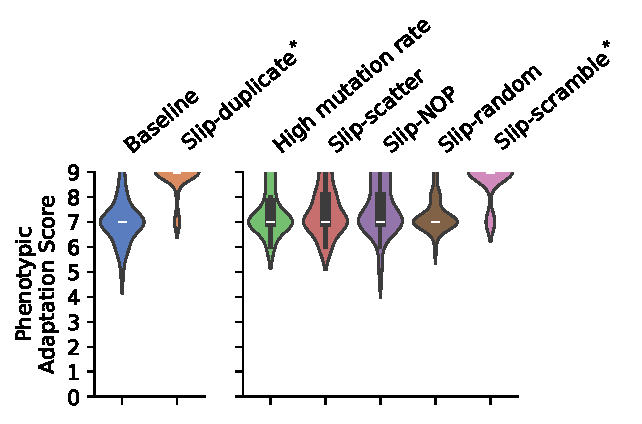
\includegraphics[
        height=4in,
        trim={0.2cm -1.5cm 0.2cm 0},
        clip
      ]{binder/binder/teeplots/col=split+env=static+hue=treatment+inner=box+kind=violin+palette=muted+viz=catplot+x=treatment+y=tasks-present+ext=.pdf}%
    \hspace*{-2.0cm}%
    \raisebox{0.125in}{%
      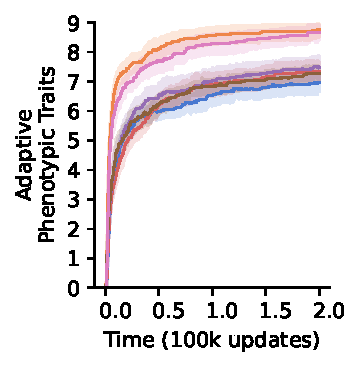
\includegraphics[
          height=2.7in,
          trim={1.36cm -0.64cm 0 0},
          clip
        ]{binder/binder/teeplots/env=static+errorbar=ci+hue=treatment+kind=line+palette=muted+viz=relplot+x=time-100k+y=tasks-present+ext=.pdf}}%
  \end{adjustbox}

  \vspace{-7ex}

  \begin{subfigure}{0.3\textwidth}
    \caption{\small slip-duplication}
    \label{fig:results_panels:slip_duplication}
  \end{subfigure}%
  \begin{subfigure}{0.35\textwidth}
    \caption{\small ablation treatments}
    \label{fig:results_panels:ablation}
  \end{subfigure}%
  \begin{subfigure}{0.22\textwidth}
    \caption{\small lineage history}
    \label{fig:results_panels:time_series}
  \end{subfigure}

  \vspace{1ex}

  \caption{\textbf{Treatments preserving slip-duplicated content facilitate adaptive evolution.}
    \small Violin plots show number of adaptive traits evolved in final dominant genotypes.
    Time series (\ref{fig:results_panels:time_series} right) shows progression of adaptive phenotypic trait counts along lineages of final dominant genotypes; color-coding corresponds to violin plots.
    Asterisk (*) markers indicate treatments with significantly more adaptive phenotypic traits compared to baseline, comparison across both \ref{fig:results_panels:slip_duplication} and \ref{fig:results_panels:ablation} panels.
    Simulation time unit is “updates,” corresponding to evaluation of ~30 genome sites per organism.}
  \label{fig:results_panels}
\end{figure}


\subsection{Sequence Content of Duplications Contribute to Adaptive Evolution}

Having observed that slip-duplicate mutations accelerate evolutionary acquisition of Logic-9 tasks in our model, we next sought to identify in greater detail which aspects of the slip duplication process contribute to facilitating adaptation using variants of the slip-duplication operator disabling or replacing a particular aspect of slip duplication.
(Figure \ref{fig:slip_mut_variants} overviews variants tested.)

As shown in Figure \ref{fig:results_panels}, we detected significant increases in adaptive evolution against baseline only for the original slip-duplicate treatment and the follow-up slip-scramble treatment --- which ablated only sequence order within duplicated regions.
Task counts under all other experimental treatments were statistically indistinguishable, or slower-adapting, compared with the baseline treatment.

Given that the slip-scramble treatment maintains the content of duplicated instruction sequences (albeit in an unordered fashion), these findings highlight how amplification of existing genetic information, in particular, promotes adaptive evolution in the study system.
In contrast to the slip-scramble and full slip-duplicate operators, other tested slip mutation variants do not duplicate information about instruction sequences already present in the genome.

Given the efficacy of the slip-scramble treatment in facilitating adaptation, we additionally tested differences in task counts between the slip-scramble and slip-duplicate treatments.
To prevent issues with multiple comparisons, we dispatched 100 new trials under both treatments for this test.

Indeed, this additional experiment confirmed that the slip-duplicate treatment did, in fact, yield higher task counts compared to the slip-scramble treatment (two-tailed Mann-Whitney U tests, W = 4305, 4028.5, 3621.5 respectively, Bonferroni-adjusted $p = 0.011$; first-phase experiments).
Thus, in our study system, it appears that the content and structure of duplicated genetic code contribute to promoting evolvability.
This finding further underscores that, specifically, the injection of existing sequence information is key to the role of gene duplication in evolution.

As above, earlier-reported experiments found the benefit to adaptive evolution from maintaining sequence order within duplicated regions generalized to changing environments where task rewards shifted with evolutionary time \citep{lalejini2017gene}.

\subsection{How Does Slip Duplication Facilitate Adaptive Evolution?}

Thus far, we have established that the locality and content of slip-duplicated genetic material both contribute substantially to its effect on facilitating adaptive evolution.
We next sought to explain \textit{how} mutations with these characteristics drive faster adaptive evolution.

In these investigations, we evaluated three hypotheses around evolutionary dynamics of slip duplications.
First, we explored how the facilitation of adaptive evolution by gene duplication differed between simple and complex traits promoted by gene duplication.
Second, we tested for signatures of evolutionary potentiation by gene duplications along lineage histories.
Finally, we examined how slip duplication influences genetic architecture with respect to brittleness and vestigial genetic material.

\subsubsection{Slip Duplication Facilitates the Evolution of Complex Traits}

\begin{figure*}
    \centering
    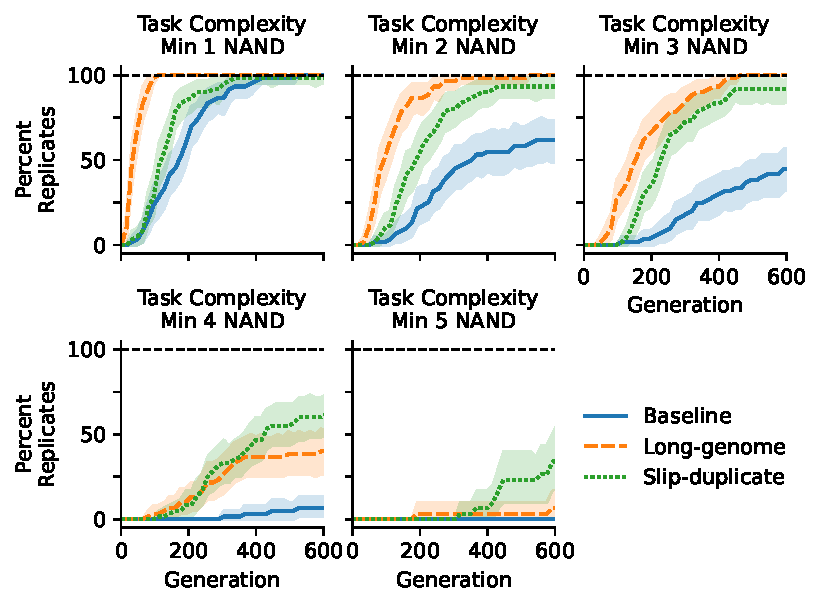
\includegraphics[width=\linewidth]{binder/binder/teeplots/adaptive-evolution-rate.ipynb/col=task-complexity+errorbar=ci+hue=treatment+kind=line+mutation=per site+post=plt-xlim-0-600+style=treatment+viz=relplot+x=generation+y=has-task+ext=.pdf}
    \caption{
        \textbf{Gene duplication boosts adaptive evolution of complex phenotypic traits.}
        \footnotesize
        Plots show fraction of replicates exhibiting available phenotypic traits, by generation from founding ancestor.
        Panels facet by trait complexity, measured by the minimum number of NAND operations required to complete the task.
        Simple tasks (top left) require only one NAND operation.
        More complex tasks (bottom right) require up to five NAND operations as shown in Figure \ref{fig:slip_mut_variants}.
        Slip-duplication treatment facilitates significantly faster adaptive evolution than long-genome treatment for the more complex tasks that require 4 or 5 subcomponents.
        Error bands give 95\% CI, bootstrapped over 30 replicates per treatment.
    }
    \label{fig:adaptive-evolution-rate}
\end{figure*}


Comparing the long-genome and baseline treatments, we observed a boost in task acquisition from increased genome length.
Disaggregating by task complexity, though, reveals that the impact of genome length is most prominent in the acquisition of simple tasks.
Figure \ref{fig:adaptive-evolution-rate} compares acquisition rates for tasks across NAND component count complexity classes --- with and without slip duplication, including the long-genome control.
The long-genome control matched or exceeded the performance of slip-duplication in evolving simple traits with 3 or fewer components.
% https://github.com/chaynes2019/AvidaGeneDupe/blob/538ede79c7301f10718ca96c8dd38782b6882632/binder/adaptive-evolution-rate.ipynb
However, slip duplication evolved the more complex 4- and 5-component traits within a significantly higher fraction of replicates compared to the long-genome control (Fisher's exact tests; 36/60 vs. 24/60, $p<0.05$ [4 components]; 10/30 vs. 2/30, $p<0.03$ [5 components]; second-phase experiments; Figure \ref{fig:adaptive-evolution-rate}).
As such, theory positing gene duplication as a catalyst for the evolution of complex traits appears to correspond well with the  behavior of our study system \citep{ohno1970evolution}.

\subsubsection{Slip-Duplicated Regions Potentiate Coding Sites for Novel Complex Traits}

% https://github.com/chaynes2019/AvidaGeneDupe/blob/4c7fa27229094adcb5bdb0b1aec541d0014b0fed/binder/hard-task-gain.ipynb
%             H-statistic       p-value
% Components
% 1              1.011820  3.144672e-01
% 2             22.787798  1.809107e-06
% 3             33.846753  5.962854e-09
% 4             15.359894  8.885441e-05
% 5              9.097744  2.559249e-03
%    Components  Prev Slip Insertion Cumulative Count      mean       std
% 0           1                                 False  0.932088  0.455109
% 1           1                                  True  1.002025  1.164197
% 2           2                                 False  0.588566  0.618479
% 3           2                                  True  1.579974  1.191681
% 4           3                                 False  0.491481  0.700256
% 5           3                                  True  1.516115  0.911430
% 6           4                                 False  0.703793  0.980105
% 7           4                                  True  1.229158  0.654042
% 8           5                                 False  0.583674  0.927917
% 9           5                                  True  1.249985  0.531423
%    Components  Prev Slip Insertion Cumulative Count  size
% 0           1                                 False    60
% 1           1                                  True    48
% 2           2                                 False    60
% 3           2                                  True    56
% 4           3                                 False    60
% 5           3                                  True    59
% 6           4                                 False    52
% 7           4                                  True    52
% 8           5                                 False    20
% 9           5                                  True    20

\begin{figure}
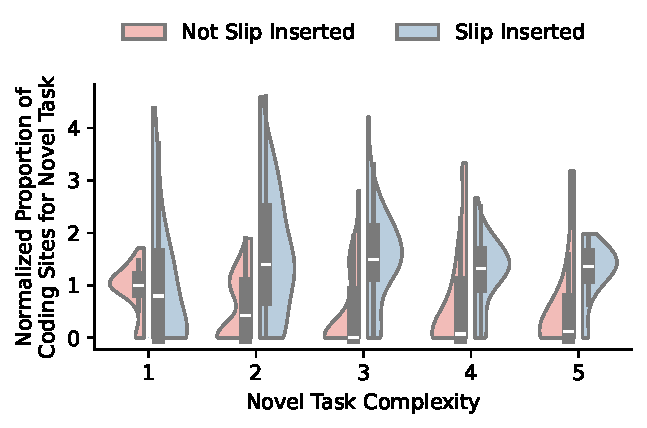
\includegraphics[
width=\linewidth
]{binder/binder/teeplots/density-norm=width+hue=prev-slip-insertion-cumulative-count+kind=violin+viz=catplot+x=components+y=is-task-coding-site+ext=.pdf}
\caption{%
  \textbf{Slip-duplicated sites are overrepresented among \textit{de novo} coding sites for complex traits.}
  \footnotesize
  Distributions compare frequencies of previously slip-duplicated and non-slip-duplicated sites among  \textit{de novo} task coding sites, normalized to neutral expectation.
  Values greater than 1 indicate that sites are overrepresented among the coding sites of novel traits compared to their background frequency.
  Differences between slip-duplicated and non slip-duplicated sites are significant for tasks requiring 2 or more NAND components (Mann-Whitney test; $p < 0.01$).
} \label{fig:potentiation}
\end{figure}


Thus far, we have established that slip duplication promotes evolution of novel traits within our study system, and that this facultative effect biases towards more complex traits.
We next sought to characterize aspects of genetic architecture through which slip duplication might drive adaptation.
In particular, we sought to understand whether the genetic material introduced through slip duplication itself is potentiated to code for novel adaptive traits.
For each first trait occurrence arising in our experiments, we assessed the fraction of new task coding sites originating in regions of the genome that had previously been slip duplicated.
Figure \ref{fig:potentiation} compares involvement in coding for new tasks between previously slip-duplicated and non-slip-duplicated sites.
For the simplest tasks, requiring only one NAND component, we found no significant difference in the likelihood of duplicated sites participating in coding regions for new tasks.
However, we found significant associations for traits with two or more NAND components (Mann-Whitney tests; all $p < 0.01$; $n=48,56,59,52,20$ observations; second-phase experiments).
Effect sizes of potentiation on likelihood to code for novel traits were $1.5\times$, $1.5\times$, $1.2\times$, and $1.2\times$ respectively for 2, 3, 4, and 5 task components.
Smaller effect sizes at 4- and 5-component tasks may be due to a larger portion of the genome becoming comprised of slip-duplicated sites (Supplementary Figure \ref{fig:potentiation-supp}), thus lowering the upper ceiling on deviation from expected.

One possible confounding factor in this result is evolutionary constraint at genome sites involved in organsims' self-replication loop.
These sites are critical to viability, with lethal outcomes when knocked out.
We found that these critical sites were less likely to be involved in slip duplication and also less likely to be involved in coding for \textit{de novo} traits.
Hence, these sites could introduce a spurious correlation between slip duplication and coding for novel tasks.
After excluding such fitness-critical sites from analysis, however, we still found similar potentiation signatures from slip duplication (Supplemental Figure \ref{fig:potentiation-supp}).

One alternative to the potentiation hypothesis is that gene duplication directly facilitates adaptation by producing mutational changes biased to discover beneficial outcomes \citep{kondrashov2012gene}.
Where regularities exist in the genotype-phenotype-fitness map, duplicated variants of existing genetic information may be more likely to encode meaningful traits.
In the fitness landscape analogy, this hypothesis would correspond to enabling steps through phenotype space that are larger, but biased to regions of viable novelty \citep{tarapore2015evolvability}.

% https://github.com/chaynes2019/AvidaGeneDupe/blob/61ea29d989ebc8ad83dcfee94f3fa556b81e3f78/binder/gain-mechanism.ipynb
In line with this possibility, we observed that a substantial fraction of gain-of-function steps on lineages directly coincided with slip duplications --- 41 of 174, or 23.6\%.
However, in these cases, sites that gained a new trait directly due to slip mutation were nonetheless more likely than chance to have been involved in earlier slip duplications (Supplemental Figure \ref{fig:potentiation-supp}).
Thus, the adaptive characteristics of slip duplication seem likely to result from a combination of potentiation and direct facilitation.

\subsubsection{Gene Duplication Accelerates Accumulation of Vestigial Coding Material}

\begin{figure}
    \centering
    \begin{subfigure}{\linewidth}
    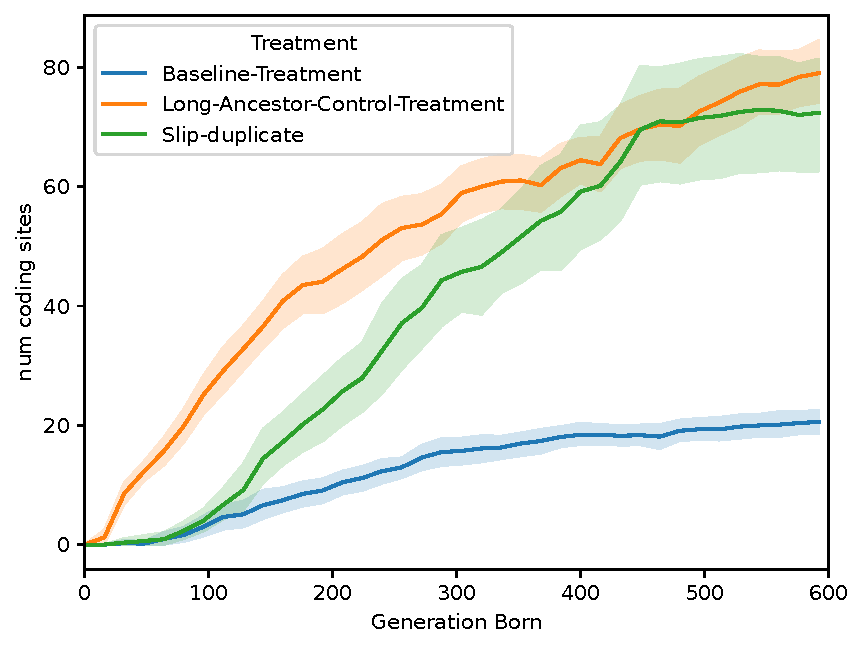
\includegraphics[width=\linewidth]{binder/binder/teeplots/hue=treatment+post=plt-xlim-0-600+viz=lineplot+x=generation-born+y=num-coding-sites+ext=.pdf}
    \caption{\footnotesize active coding sites}
    \label{fig:num-coding-sites:active}
    \end{subfigure}

    \begin{subfigure}{\linewidth}
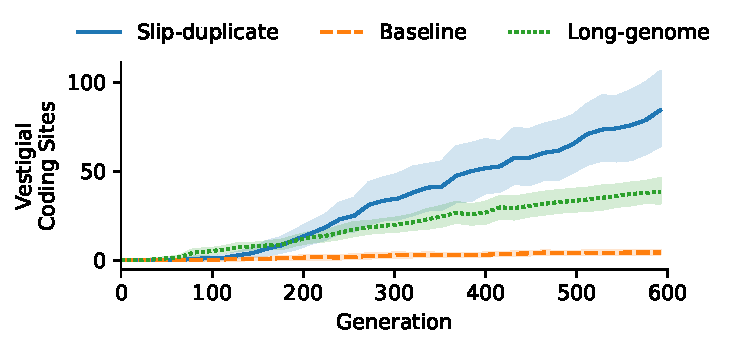
\includegraphics[width=\linewidth,clip, trim=0 0 0 0.8cm]{binder/binder/teeplots/hue=treatment+post=plt-xlim-0-600+viz=lineplot+x=generation-born+y=num-free-sites+ext=.pdf}
    \caption{\footnotesize vestigial coding sites}
    \label{fig:num-coding-sites:vestigial}
    \end{subfigure}
    \caption{
        \textbf{Gene duplication boosts accumulation of vestigial coding sites.}
        \footnotesize
        Generation-by-generation counts of coding sites over evolutionary history.
        Here, ``active'' coding sites refer to genome instructions determined through knockout to contribute to fitness with respect to self-copy viability or a rewarded phenotypic trait.
        As shown in panel \ref{fig:num-coding-sites:active}, gene duplication yields active coding site counts comparable to long-genome control.
        Vestigial coding site count, by contrast, reports the number of sites determined to have contributed to fitness in an ancestor, but are no longer active coding sites.
        As shown in panel \ref{fig:num-coding-sites:active}, vestigial coding site count under slip-duplication treatment outpace control treatments.
        Error bands give 95\% CI, bootstrapped over 30 replicates per treatment.
    }
    \label{fig:num-coding-sites}
\end{figure}


In a final set of analyses, we broadened the scope of inquiry beyond trait acquisition to assess the consequences of gene duplication with respect to whole-genome architecture.
Our focus within this purview was on genome robustness, which we defined in terms of sensitivity of fitness to individual mutations \citep{lenski1999genome}.
That is, we measured robustness in terms of ``brittleness'' the number of genome sites ``critical'' to fitness, where a single-site knockout induces loss of replicator viability or one or more adaptive phenotypic traits (i.e., tasks).
We used Avida's genome evaluator tool to identify and quantify such ``fitness-critical'' sites.\footnote{%
Although sufficiently representative for our purposes, limitations exist in detecting Avida genome functionality through single-site knockouts; such an approach can underestimate aspects of genome sequence complexity involving small effects or redundancy \citep{lenski1999genome,moreno2024cryptic}.
}

One conventional perspective on gene duplication is \textit{vis-a-vis} facilitation of neutral dynamics, wherein copied genetic material reduces brittleness by introducing redundancies \citep{wagner1996genetic}.
To assess the relevance of this perspective in our study system, we performed slip-duplicate mutational assays to quantify the baseline distribution of slip insertion mutations on genome brittleness, in the absence of selection.
Specifically, we generated possible slip duplications applied to final-dominant genome lineages evolved under the slip-duplicate treatment, and filtered our sample to exclude slip duplications that affected self-replication viability or altered the task-performance phenotype.
These analyses confirmed that fitness-neutral slip insertions did indeed tend to reduce the number of genome sites detectable as a single point of failure for performed tasks.
% https://github.com/chaynes2019/AvidaGeneDupe/blob/9fee1f13a8d31f25d1dd799c6a26f9b7fa617738/binder/indel-effect-nulldist.ipynb
On average, we found that neutral slip insertions decreased coding site count by 6.8 sites (bootstrapped 95\% CI 6.4 to 7.3).
This effect was strongest in genomes with high complexity; for instance, neutral insertion mutations decrease coding site count by 9.2 and 8.3 sites on average in genomes that encode 4- and 5-component complexity tasks, respectively (bootstrapped 95\% CIs 8.5 to 9.9 and 7.2 to 9.3).
Supplementary Figure \ref{fig:nulldist} presents these results.

% https://github.com/chaynes2019/AvidaGeneDupe/blob/binder/binder/gain-mechanism.ipynb
To assess the consequences of this bias towards redundancy, we next pivoted to assess coding site accumulation within genomes over the course of evolution.
Counter to naive expectation, we found that the slip duplication treatment accrued fitness-critical sites at a generation-on-generation rate comparable to the long-genome baseline treatment, rather than decreasing net brittleness (Figure \ref{fig:num-coding-sites:coding}; Mann-Whittney test, $U=361$, $p=0.19$; second-phase experiments).
Despite this similarity, however, when measurements were taken inclusive of vestigial coding sites (those which had \textit{previously} been fitness-critical earlier within a lineage), we found a significantly increased coding site count associated with the slip-duplicate treatment (Mann-Whittney test, $U=630$, $p<0.01$; second-phase experiments).
Figure \ref{fig:num-coding-sites:coded} compares vestigial-inclusive coding site counts trajectories along final-dominant lineages.
In sum, within our study system, gene duplication processes increased the net supply of coding material in the genome available to neutral processes, but the accumulation of critical sites representing single points of failure remained substantially unaffected.

% One possible explanation is that selective pressures are driving the two treatments to reach a similar number of critical sites, but slip duplication can duplicate and copy genome content in a manner that increases the copy count of previously coding sites relative to the number of critical sites.
